A seguito di una prima parte teorica introduttiva, si procede in questo capitolo con la presentazione 
dell'impostazione pratica che si è voluto dare alle sperimentazioni condotte. La struttura secondo la quale verranno esposte 
le informazioni nei seguenti paragrafi ricalca la partizione logica alla base del codice sviluppato, pragmaticamente diviso 
in quattro moduli tra loro indipendenti:
\begin{itemize}
    \item Generazione dei parametri
    \item Generazione delle istanze di problemi MIP
    \item Risoluzione delle istanze di problemi
    \item Estrazione ed analisi dei risultati
\end{itemize}



%----------------------------------NEW SECTION

\section{Generazione dei parametri}
\label{sec:pargen}
Il primo problema presentatosi è stato quello relativo all'individuamento dei parametri di flusso e distanza, in quanto 
fondamentali per la creazione di istanze del problema e conseguentemente anche per la loro risoluzione.

La prima possibilità valutata è stata la generazione di valori casuali per comporre le matrici dei parametri $A$ e $B$. 
Questa però è stato scartata fin da subito poichè utilizzare valori di tale tipologia non permette di fornire una versione 
pseudo-realistica di istanze del problema ed inoltre, non garantisce alcun tipo di uniformità nella generazione delle istanze, 
il che non ci permette di effettuare successivamente uno studio approfondito sulla loro complessità di risoluzione.

La soluzione a questo problema è stata individuata in un metodo illustrato in un articolo del professor Éric D. Taillard del 1995
\cite{TAILLARD}. Come verrà illustrato più nello specifico nella prossima sezione, il metodo utilizzato è detto Densità di
grigio, in inglese (\textit{Density of grey}). Esso, oltre a compensare i difetti del metodo di istanziamento casuale, permette
di automatizzare la creazione delle matrici dei parametri realizzando un algoritmo che richiede ai fini della generazione 
esclusivamente due valori: dimensione dell'istanza e densità utilizzata.

Come anticipato nell'introduzione, per realizzare tale processo è stato fatto uso del linguaggio di programmazione \textit{Python} 
\cite{python} e come supporto \textit{NumPy} \cite{NumPy}, una libreria open source che aggiunge supporto a grandi matrici 
e array multidimensionali insieme a una vasta collezione di funzioni matematiche di alto livello per poter operare efficientemente 
su queste strutture dati.

\subsection{Istanze Tai*c}
\label{subsec:taic}
Le istanze Tai*C, la cui denominazione deriva dal nome del loro ideatore, sono una particolare classe di problemi di assegnamento quadratico
che si fondano sull'utilizzo del metodo di Densità di grigio, il quale può essere descritto nel seguente modo.

Al fine di ottenere una tonalità di grigio di densità pari a $m/n$ , il metodo in questione consiste nel generare una griglia 
rettangolare contenente $n = n_1 \times n_2$ caselle quadrate, $m$ delle quali sono nere e $n-m$ sono bianche. 
Giustapponendo molte di queste griglie è possibile ottenere una superficie grigia di gradazione pari a $m/n$.
Per ottenere la miglior qualità di colore, è necessario che le caselle nere, o quelle bianche, siano sparse uniformemente nella griglia.

A prova di ciò viene qui riportata un'applicazione del metodo realizzata con una delle soluzioni ottenute.
\begin{figure}[h!]
    \centering
    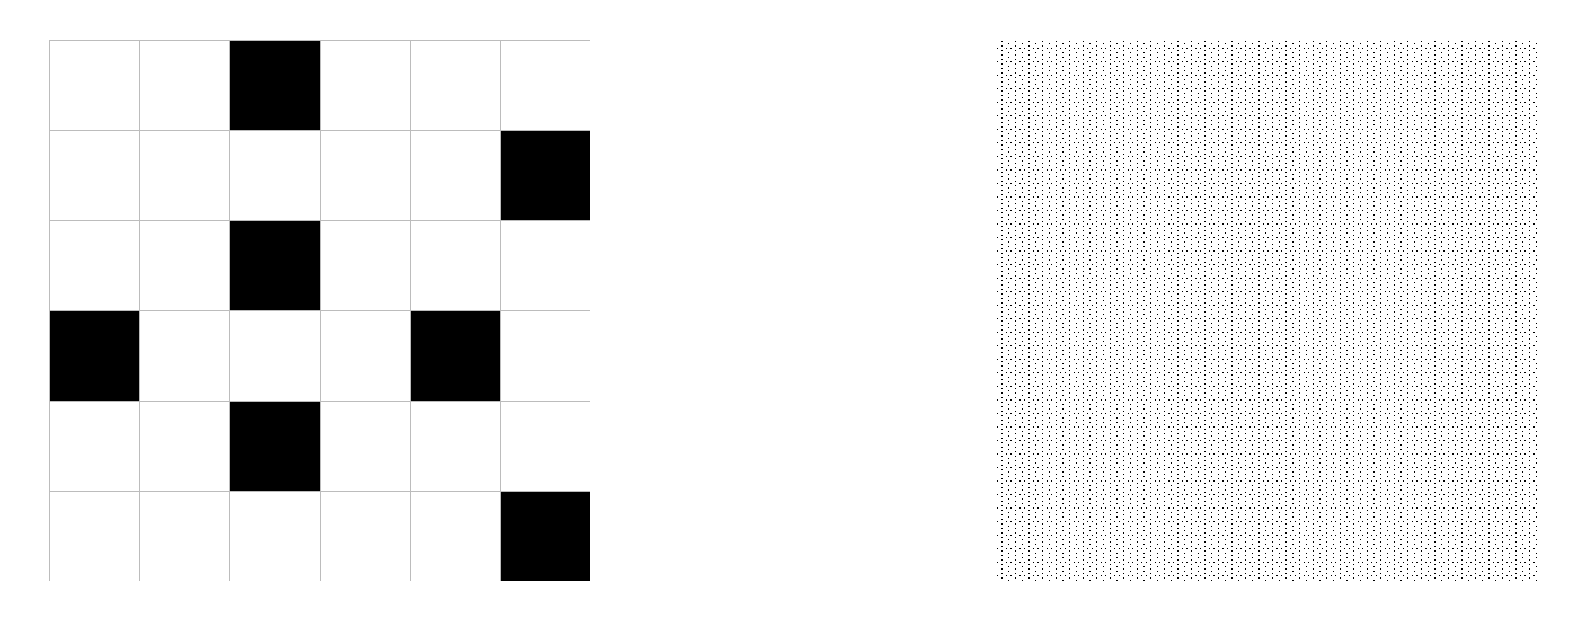
\includegraphics[scale=0.21]{images/Density_of_Grey.png}
    \caption{a sinistra la griglia relativa ad una soluzione ottima di un'istanza \textit{Tai36c} a densità $d=30\%$, 
             \newline a destra quella ottenuta accostando $1600$ griglie del tipo a sinistra}
    \label{fig:dnsgry}
\end{figure}

Per rendere al meglio l'idea che sta alla base del metodo, è possibile paragonare le caselle nere a degli elettroni e la griglia 
allo spazio accessibile agli elettroni. Il posizionamente di quest'ultimi deve essere effettuato in modo tale che la somma delle 
intensità delle forze di repulsione elettrostatica è minimizzata.

Nei problemi considerati, le forze $f_{rstu}$ $\(r,t \in \[1,n_1\] \; s,u \in \[1,n_2\]\)$ presenti tra le caselle $i$ e $j$
locate rispettivamente nelle posizioni della griglia di coordinate $\(r,s\)$ e $\(t,u\)$ sono definite come segue:
\begin{align*}
    f_{rstu} \, = \, \max_{v,w \,\in\, \{-1,0,1\}} \frac{1}{\(r-t+n_1 v\)^2 + \(s-u+n_2 w\)^2}
\end{align*}

Per ottenere una densità di grigio pari a $m/n$ è possibile risolvere un problema di tipo $QAP$ (assegnamento quadratico) in cui 
i parametri sono definiti nel seguente modo.
\begin{align*}
    a_{ij} \, = \, \begin{cases} 1 & \mbox{if } i \leq m \mbox{ and } j \leq m \\ 0 & \mbox{otherwise} \end{cases} 
    \qquad \;\;
    b_{ij} \,=\, b_{\; n_2 \(r-1\)+s \;\; n_2\(t-1\)+u} \,=\, f_{rstu}
\end{align*}

La $i$-esima componente $\(i\leq m\)$ di una soluzione $\pi$, $\pi_i = \pi_{n_2 \(r-1\)+s}$ fornisce la posizione in cui
deve essere posizonata una casella nera.

Nonostante la relativa semplicità di questi problemi, molti metodi risolutivi potrebbero non funzionare correttamente a causa 
dell'esistenza di più soluzioni con lo stesso valore obiettivo. Tali soluzioni posso essere ottenute scambiando la posizione 
di due caselle nere oppure attuando rotazioni, traslazioni o simmetrie delle caselle nella griglia. Queste tre infatti,
sono azioni che non mutano il valore della soluzione associata.

Questi problemi sono identificati in letteratura dalla sigla $grey$n$_1\_$n$_2\_$m e sono stati risolti pseudo-ottimamente 
fino a valori $n_1 = n_2 = 8$. Scegliendo definizioni dei parametri di distanza differenti oppure variando le scelte prese sui 
valori $n_1$, $n_2$ ed $m$ è possibile ottenere moltissime varianti del problema.

A questo punto è possibile sfruttare le definizioni degli elementi che caratterizzano questo modello, per realizzare degli algoritmi 
che generino la matrice dei flussi $A$ e quella delle distanze $B$ sulla base dei soli tre parametri richiesti, le dimensioni $n_1$ e $n_2$ 
(si ricorda queste sono in relazione con la dimensione dell'istanza $n$ nel seguente modo: $n=n_1\times n_2$) e la densità di grigio 
utilizzata $d$. 

Qui di seguito sono riportati gli pseudocodici degli algoritmi in questione insieme a quello delle eventuali funzioni che sono state 
utilizzate all'intero di essi.

\begin{algorithm}
    \caption{Matrix A generation}\label{A_gen}
    \begin{algorithmic}[1]
    \Function{A-generator}{$n, \,d$}
    \State $* \quad sia\; A = \[a_{ij}\] \quad *$
    \State $m \gets round\(n\cdot \(d/100\)\)$
    \ForAll{$i \in [0,n)$}
    \ForAll{$j \in [0,n)$}
        \If{$i<m \;\text{or}\; j<m$} \State $a_{ij} \gets 1$
        \Else \State $a_{ij} \gets 0$
        \EndIf
    \EndFor
    \EndFor
    \Return $A$
    \EndFunction
    \end{algorithmic}
\end{algorithm}

\begin{algorithm}
    \caption{Matrix B generation}\label{B_gen}
    \begin{algorithmic}[1]
    \Function{Force}{$n_1,\, n_2,\, r,\, s,\, t,\, u$}
    \State $max \gets 0$
    \ForAll{$v \in \{-1, 0, 1\}$}
    \ForAll{$w \in \{-1, 0, 1\}$}
        \State $m \gets 1\,/\(\(r-t+n_1 v\)^2 + \(s-u+n_2 w\)^2\)$
        \State $max \gets \max \(max, m\)$
    \EndFor
    \EndFor
    \Return $max$
    \EndFunction
    \BState
    \Function{B-generator}{$n_1,\, n_2$}
    \State $* \quad sia\; B = \[b_{ij}\] \,con \;valori \;inizializzati \;a \;zero \quad *$
    \State $scale \gets 100000$
    \ForAll{$r \in [0,n_1)$}
    \ForAll{$s \in [0,n_2)$}
    \ForAll{$t \in [0,n_1)$}
    \ForAll{$u \in [0,n_2)$}
        \State $i \gets n_2 \cdot \(r-1\)+s$
        \State $j \gets n_2 \cdot \(t-1\)+u$
        \If{$b_{ij} \, \neq \, 0$} \State continue
        \Else 
            \State $b_{ij} \gets \text{round} \(\text{Force}\(n_1,n_2,r,s,t,u\)\cdot scale\)$
            \State $b_{ji} \gets b_{ij}$
        \EndIf
    \EndFor
    \EndFor
    \EndFor
    \EndFor
    \Return $B$
    \EndFunction
    \end{algorithmic}
\end{algorithm}

Come si può intuire osservando lo pseudocodice del primo algoritmo, nella sua costruzione è stata presa la decisione di 
esprimere la densità $d$ in punti percentuali, ovvero $d \in \[0,100\]$. Da qui il perchè nel calcolo del valore di $m$ è necessaria 
la divisione per $100$.

Relativamente al secondo algoritmo invece, sono necessarie alcune puntualizzazioni. Alla riga n°20 si può notare come il valore della distanza 
calcolata tramite la funzione \textit{Force} non avviene direttamente ma vengono effettuate delle operazioni intermedie. Come prima cosa 
il valore ritornato dalla funzione viene scalato di un fattore \textit{scale} pari a $100000$ e successivamente viene arrotondato all'intero 
più vicino. In tale modo è stato possibile confrontare le matrici ottenute, nello specifico la \textit{Tai64c} e la \textit{Tai256c}, 
con quelle messe a disposizione dal sito web \textit{QAPLIB} \cite{QAPLIB}, una libreria online contenente diverse tipologie di istanze 
di prolemi di assegnamento quadratico tra cui la \textit{Tai*c}. Quest'operazione ha permesso in fase di costruzione dell'algoritmo di 
garantirne la correttezza. All riga n°21 invece, si sfrutta la proprietà di simmetria della matrice $B$ per risparmiare 
metà dei calcoli dei valori di distanza, riducendo così la complessità temporale dell'algoritmo. Si ricorda infatti che, date due unità 
qualsiasi, la distanza della prima dalla seconda è la medesima della seconda dalla prima.

Come si può notare sono state utilizzate due funzioni di cui non è stato riportato lo pseudocodice, \textit{max} e \textit{round}.
Questo perchè sono due funzioni elementari messe a disposizione della libreria standard di \textit{Python} \cite{python} di cui il 
funzionamento è noto. La prima richiede due valori come parametri e ritorna il massimo tra questi mentre la seconda ritorna 
l'arrotondamento all'intero più vicino del numero fornito come parametro.



%----------------------------------NEW SECTION
\newpage
\section{Generazione delle istanze di problemi MIP}
Terminata la generazione delle matrici dei parametri, costituenti il \textit{dataset} grezzo alla base di questo lavoro, è stato necessario ricavare a 
partire da ciascuna coppia di matrici $A$ e $B$ il corrispondente problema di programmazione lineare intera di assegnamento quadratico. Per fare questo è stato 
inizialmente necessario ricavare una modellazione algebrica del problema stesso, definendo variabili, vincoli e funzione obiettivo con cui 
rappresentarlo formalmente. Come sarà possibile vedere successivamente, a tale modello è stato necessario apportare diverse modifiche per renderlo
prima corretto e poi anche ottimizzato. Solo in un secondo momento è stato quindi possibile procedere con l'implementazione del modello nel software 
e la costruzione delle singole istanze, facendo uso di un'apposita libreria Python.

\subsection{Modellazione algebrica}
Un \textit{modello algebrico} di un problema di programmazione lineare intera è un modello che descrive le caratteristiche della soluzione 
ottima al problema mediante relazioni matematiche \cite{rop}. Un modello algebrico è composto dai seguenti elementi:
\begin{itemize}
\item \textsl{insiemi}, i quali racchiudono gli elementi del sistema permettendo l'indicizzazione delle grandezze trattate nel problema
\item \textsl{parametri}, ossia quantità costanti e definite nella formulazione del problema stesso, che solitamente sono delle proprietà relative agli insiemi definiti precedentemente
\item \textsl{variabili}, ossia le grandezze incognite del sistema, su cui l'algoritmo può agire (nei limiti imposti dai vincoli dal loro dominio) per ottimizzare il valore della soluzione
\item \textsl{vincoli}, ossia relazioni matematiche che permettono di verificare l'ammissibilità delle soluzioni e, di conseguenza, definire quali assegnazioni alle variabili sono accettabili nel contesto del problema e quali invece non lo sono
\item \textsl{funzione obiettivo}, che permette la traduzione di una soluzione del problema in un valore numerico, rendendone possibile di conseguenza l'ottimizzazione
\end{itemize}

Un modello algebrico di un problema di programmazione lineare permette quindi la definizione in forma dichiarativa delle caratteristiche della soluzione cercata, 
piuttosto che definire una strategia con cui eseguire la ricerca della soluzione stessa. Un modello di programmazione matematica potrebbe essere quindi paragonato 
ad un linguaggio dichiarativo, che descrive il risultato che si vuole ottenere, piuttosto che ad un linguaggio procedurale, che indica invece la sequenza di passi 
da percorrere per arrivare a quel risultato.

Durante la fase di modellazione formale del problema viene persa parte della potenza descrittiva caratteristica del linguaggio naturale, a vantaggio però della 
possibilità di utilizzare algoritmi particolarmente efficienti nella risoluzione dello stesso, che possono essere applicati solo quando il problema è definito in questa forma.

Come si vedrà nel prosieguo della trattazione, nel caso del problema analizzato in questo lavoro la modellazione algebrica non è stata di immediata risoluzione.

\noindent
Per prima cosa sono stati identificati gli insiemi del problema, ovvero
\begin{align*}
I \, &: \, \mbox{insieme delle posizioni (\textit{locations})} \\
U \, &: \, \mbox{insieme delle unità (\textit{facilities})}
\end{align*}
Per quanto riguarda l'identificazione dei parametri, quest'operazione è già stata trattata nella sezione precedente e rappresenta le 
fondamenta su cui l'istanze del problema vengono costruite. Facendo uso degli algoritmi appositamente costruiti è possibile ottenere 
tutti i parametri necessari in forma matriciale del tipo:
\begin{align*}
A = \[a_{uv}\] \quad & \mbox{con} \; a_{uv} : \, \mbox{flusso dall'unità \textit{u} all'unità \textit{v}} \\
B = \[b_{ij}\] \quad & \mbox{con} \; b_{ij} : \, \mbox{distanza dalla posizione \textit{i} alla posizione \textit{j}}
\end{align*}

Per quanto concerne le variabili del problema, queste sono indicizzate dall'insieme delle unità $I$ e da quello delle posizioni $U$ e la loro definizione è la seguente:
\begin{align*}
x_{iu} = \begin{cases}  1 & \mbox{se l'unità } u \in U \mbox{ è stata assegnata alla posizione } i \in I\\ 0 & \mbox{altrimenti} \end{cases}
\end{align*}
È stato inoltre necessario definire due vincoli per assicurare la correttezza della soluzione trovata. Il primo garantisce che ogni unità venga assagnata ad esattamente una posizione e il secondo invece, che ogni posizione sia asseganta ad esattamente un'unità.
\begin{align*}
    \sum_{i\in I} x_{iu} = 1 \quad & \forall u \in U \\
    \sum_{u\in U} x_{iu} = 1 \quad & \forall i \in I
\end{align*}

Infine, la funzione obiettivo $f(x)$, che dovrà essere minimizzata dal risolutore, viene definita come segue.
\begin{align*}
    f\(x\) \, = \, \min \, \sum_{i\in I} \sum_{u\in U} \sum_{j\in I} \sum_{v\in U} \, a_{uv}\cdot b_{ij}\cdot x_{iu}\cdot x_{jv}
\end{align*}

Il modello algebrico del problema di assegnamento quadratico ricavato, può dunque essere complessivamente definito nel seguente modo: 
\begin{align}
    \label{eq:mipqap}
	\begin{array}{l}
      \min \, \sum_{i\in I} \sum_{u\in U} \sum_{j\in I} \sum_{v\in U} \, a_{uv}\cdot b_{ij}\cdot x_{iu}\cdot x_{jv} \\
      \sum_{i\in I} \, x_{iu} = 1\,\qquad \forall\; u \in U \\
      \sum_{u\in U} x_{iu} = 1     \qquad \forall\; i \in I \\
      x_{iu} \in \{0,1\}           \;\;\,\qquad \forall \; i \in I ,\; u \in U
    \end{array}
\end{align}


\subsection{Linearizzazione del modello}
\label{subsec:lin}
Come è possibile notare, il modello algebrico ricavato precedentemente (\ref{eq:mipqap}) non rispetta completamente i canoni della 
formulazione dei problemi di programmazione lineare intera (\ref{eq:mip}). Ai fini della risoluzione del problema, è dunque necessario 
ricondurre il modello in oggetto alla formulazione \textit{MIP} apportando alcune modifiche necessarie.

Nello specifico il problema risiede nella funzione obiettivo. Come lascia intuire il nome, la programmazione lineare 
intera esige un funzione obiettivo lineare, mentre in quella del modello in questione è presente il prodotto fra incognite 
$\(x_{iu}\cdot x_{jv}\)$ che la rende non lineare.

Il problema è stato risolto effettuando un'operazione di linearizzazione. Tale processo consiste nell'introduzione di una variabile
$y_{iujv}$ che vada a sostituire il prodotto fra variabili, rendendo così lineare la funzione obiettivo.

\noindent
Tale variabile è stata definita nel seguente modo:
\begin{align*}
    y_{iujv} \, = \, x_{iu}\cdot x_{jv}
\end{align*}
Tuttavia, affinchè questa variabile sia consistente con i valori delle variabili $x_{iu}$ e $x_{jv}$ che la definiscono è stato necessario 
introdurre tre ulteriori vincoli.
\begin{align*}
    y_{iujv} \,& \leq \, x_{iu}   \;\;\;\qquad \forall \; i,j \in I ,\; u,v \in U \\ 
    y_{iujv} \,& \leq \, x_{jv}   \;\;\;\qquad \forall \; i,j \in I ,\; u,v \in U \\
    y_{iujv} \,& \geq \, x_{iu} + x_{jv} - 1 \qquad \forall \; i,j \in I ,\; u,v \in U 
\end{align*}
I vincoli sopra elencati garantiscono che la variabile $y_{iujv}$ assuma valore $1$ se e solamente se entrambe le variabili 
$x_{iu}$ e $x_{jv}$ assumono valore $1$. Nel caso in cui anche solo una di esse dovesse assumere valore $0$, anche $y_{iujv}$ 
assumerebbe valore $0$.

Pragmaticamente, la variabile qui introdotta indica se l'unità $u$ è stata assegnata alla posizione $i$ e contemporaneamente 
l'unità $v$ è stata assegnata alla posizione $j$ o meno.

Tenendo conto delle nuove modifiche e l'aggiunta dei nuovi vincoli, il modello complessivo corrisponde al seguente.
\begin{align}
    \label{eq:mipqaplin}
	\begin{array}{l}
      \min \, \sum_{i\in I} \sum_{u\in U} \sum_{j\in I} \sum_{v\in U} \, a_{uv}\cdot b_{ij}\cdot y_{iujv} \\
      \sum_{i\in I} \; x_{iu} = 1  \qquad \forall u \in U \\
      \sum_{u\in U} x_{iu} = 1     \qquad \forall i \in I \\
      y_{iujv} \, \leq \, x_{iu}   \;\;\;\qquad \forall \; i,j \in I ,\; u,v \in U \\ 
      y_{iujv} \, \leq \, x_{jv}   \;\;\;\qquad \forall \; i,j \in I ,\; u,v \in U \\
      y_{iujv} \, \geq \, x_{iu} + x_{jv} - 1      \qquad \forall \; i,j \in I ,\; u,v \in U  \\
      x_{iu} ,\, y_{iujv} \in \{0,1\}   \;\,\,\quad\qquad \forall \; i,j \in I ,\; u,v \in U
    \end{array}
\end{align}
A questo punto della trattazione è doveroso effettuare un'importante osservazione. Come si può notare la variabile principale 
presente nella funzione obiettivo, ovvero quella introdotta in questa sezione, è indicizzata da quattro elementi tutti appartenenti 
a insiemi caratterizzati dalla medesima cardinalità, che per praticità indicheremo con la lettera \textit{n}. 

Ciò implica che dato \textit{n}, numero totale delle posizioni e delle unità, vanno prese in esame $n^4$ variabili differenti 
e, come è facilmente intuibile, questo comporta pesanti conseguenze a livello di complessità computazionale nella risoluzione 
del problema. Si riportano qui di seguito alcuni esempi che evidenziano la questione.
\begin{align*}
    n=4  \;\;&\Rightarrow\;\; \mbox{n° variabili} = 4^4 = 256 \\
    n=9  \;\;&\Rightarrow\;\; \mbox{n° variabili} = 9^4 = 6561 \\
    n=16 \;\;&\Rightarrow\;\; \mbox{n° variabili} = 16^4 = 65536
\end{align*}
Nonostate la potenza computazionale non indifferente dell'hardware che è stato messo a dispozione per effettuare gli esperimenti, 
questo rapporto tra numero di variabili e cardinalità degli insiemi non permette di spingersi molto in avanti con la dimensione delle 
istanze nelle sperimentazioni. Senza apportare alcuna semplificazione al modello, non sarebbe stato possibile raccogliere dati a 
sufficienza per realizzare uno studio approfondito.

\subsection{Semplificazione del modello}
È possibile notare che l'ultima versione del modello (\ref{eq:mipqaplin}) è valida per qualunque problema di assegnamento quadratico. 
Tuttavia, come è stato mostrato nella sezione \ref{sec:pargen}, per generare i valori dei parametri di flusso e distanza è stata presa 
la decisione di considerare una classe di problemi \textit{QAP} specifica, la classe Tai*C.

Un modo che potesse semplificare il modello, riducendo quindi il numero di variabili rispetto alla dimensione delle istanze, senza 
alterarne la validità, è stato trovato sfruttando le caratteristiche della classe di istanze considerata. 

Nello specifico, sono state utilizzate le proprietà della matrice dei flussi $A=\(a_{ij}\)$. \newline
Si ricorda che il singolo parametro $a_{ij}$ è definito nel seguente modo:
\begin{align*}
    a_{ij} \, = \, \begin{cases} 1 & \mbox{if } i \leq n_1 \mbox{ and } j \leq n_1 \\ 0 & \mbox{otherwise} \end{cases}
\end{align*}
dove $\; n_1 =n\cdot d\leq n \;$ è il numero di caselle nere nella griglia di generazione.

\noindent
Di conseguenza, la struttura della matrice $A$ è la seguente.
\begin{align*}
    A \; = \;
    \begin{bmatrix}
        1 & 1 & . & 1 & 0 & . & 0 \\
        1 & . & . & 1 & 0 & . & 0 \\
        . & . & . & . & . & . & . \\
        1 & 1 & . & 1 & 0 & . & . \\
        0 & 0 & . & 0 & 0 & . & 0 \\
        . & . & . & . & . & . & . \\
        0 & 0 & . & . & 0 & . & 0
    \end{bmatrix}
\end{align*}
Si nota che solo i valori appartenenti al quadrante $n_1\times n_1$ in alto a sinistra hanno valore unitario, mentre tutti gli altri 
hanno valore nullo. È quindi possibile definire un nuovo metodo di indicizzazione delle unità sulla base del loro flusso. 
Data l'unità $i \in I$:
\begin{align*}
        m_i \,=\, 
        \begin{cases}
            1 & \mbox{if } i \leq n_1 \\ 2 & \mbox{otherwise}
        \end{cases}
        \quad\qquad m_i \, \in \, M
\end{align*}

\newpage \noindent
A questo punto esistono esclusivamente due tipologie di unità. Pertanto è possibile ridurre la matrice dei flussi alla seguente 
matrice $2\times 2$:
\begin{align*}
    A \; = \;
    \begin{bmatrix}
        1 & 0 \\
        0 & 0
    \end{bmatrix}
\end{align*}
Conseguentemente, muta anche la definizione delle variabili del problema.
\begin{align*}
    x_{im} = \begin{cases}  1 & \mbox{se l'unità di categoria } m \mbox{ è stata assegnata alla posizione } i \in I\\ 0 & \mbox{altrimenti} \end{cases}
\end{align*}
Infine, per garantire la correttezza del modello è necessario aggiungere i seguenti vincoli che garantiscono la corrispondenza tra 
la vecchia e la nuova matrice dei flussi.
\begin{align*}
    \begin{array}{l}
        \sum_{i\in I} \, x_{im} = n_1    \qquad\qquad m=1\\
        \sum_{i\in I} \, x_{im} = n-n_1  \,\qquad m=2
    \end{array}
\end{align*}
È facilmente dimostrabile che il secondo vincolo è rindondante in quanto è garantito dal primo. Per questo motivo verrà omesso dalle 
versione successive del modello algebrico.

\noindent
Trascurando momentaneamente la linearizzazione, il modello comprensivo delle ultime modifiche è il seguente.
\begin{align*}
	\begin{array}{l}
      \min \, \sum_{i\in I} \sum_{m\in M} \sum_{j\in I} \sum_{p\in M} \, a_{mp}\cdot b_{ij}\cdot x_{im}\cdot x_{jp} \\
      \sum_{i\in I} \, x_{im} = n_1    \qquad\qquad m=1\\
      x_{im} \in \{0,1\}           \;\;\,\qquad \forall \; i \in I ,\; m \in M
    \end{array}
\end{align*}
A questo punto si può notare come a dare un contributo non nullo alle sommatorie siano solamente i prodotti relativi alle 
coppie di unità appartenenti entrambe alla categoria $m=1$, per le quali infatti si ha $a_{mp}=a[1,1]=1$. Negli altri casi il flusso 
a valore nullo azzera il prodotto rendendo l'intero addendo nullo. 

Per questo motivo è possibile semplificare ulteriormente il modello omettendo i valori di flusso e l'indicizzazione delle variabili 
rispetto alle unità. 

\newpage \noindent
In tal modo si ottiene il seguente risultato:
\begin{align*}
    x_{i} = \begin{cases}  1 & \mbox{se un unità di categoria 1} \mbox{ è stata assegnata alla posizione } i \in I\\ 0 & \mbox{altrimenti} \end{cases}
\end{align*}
e per quanto riguarda il modello,
\begin{align*}
	\begin{array}{l}
      \min \, \sum_{i\in I} \sum_{j\in I} \, b_{ij}\cdot x_{i}\cdot x_{j} \\
      \sum_{i\in I} \, x_{i} = n_1 \\
      x_{i} \in \{0,1\}           \;\;\,\qquad \forall \; i \in I
    \end{array}
\end{align*}
Linearizzando il modello precedente con le stesse modalità illustrate nella sezione \ref{subsec:lin}, è possibile ottenere la versione 
finale del modello algebrico del problema.
\begin{align}
    \label{eq:mipqapfinal}
	\begin{array}{l}
      \min \, \sum_{i\in I} \sum_{j\in I} \, b_{ij}\cdot y_{ij} \\
      \sum_{i\in I} \, x_{i} = n_1 \\
      y_{ij} \, \leq \, x_{i}   \;\;\;\qquad \forall \; i,j \in I \\ 
      y_{ij} \, \leq \, x_{j}   \;\;\;\qquad \forall \; i,j \in I \\
      y_{ij} \, \geq \, x_{i} + x_{j} - 1      \qquad \forall \; i,j \\
      x_{i} ,\, y_{ij} \in \{0,1\}      \;\quad\qquad \forall \; i,j \in I
    \end{array}
\end{align}
In questo caso, a differenza del modello nella versione (\ref{eq:mipqaplin}), le variabili della funzione obiettivo $y_{ij}$ sono 
indicizzate su soli due elementi, entrambi appartenti allo stesso insieme di cardinalità $n$. Ciò implica che dato il numero di possibili posizioni $n$, 
cardinalità di $I$, verranno  prese in esame $n^2$ variabili differenti e non più $n^4$. È stato dunque ottenuto un guadagno di due ordini di grandezza sul numero 
di variabili, garantendo così la possibilità di risolvere, tramite l'hardware e i software messi a disposizione, istanze del problema di grandezza 
sufficientemente elevata da poterne realizzare uno studio.


\subsection{Modellazione nel software}
prova




%----------------------------------NEW SECTION

\section{Risoluzione delle istanze di problemi}
prova




%----------------------------------NEW SECTION

\section{Estrazione ed analisi dei risultati}
prova